%% LyX 2.1.3 created this file.  For more info, see http://www.lyx.org/.
%% Do not edit unless you really know what you are doing.
\documentclass[english]{article}
\usepackage[latin9]{inputenc}
\usepackage{amsmath}
\usepackage{graphicx}

\makeatletter
%%%%%%%%%%%%%%%%%%%%%%%%%%%%%% User specified LaTeX commands.
\usepackage[margin=0.75in]{geometry} % see geometry.pdf on how to lay out the page. There's lots.
\usepackage{graphicx}
\usepackage{cleveref}
\usepackage{amsmath}
\usepackage{multirow}
\usepackage{listings}
\usepackage{color}
\usepackage{CJK}
\definecolor{mygreen}{RGB}{28,172,0}
\definecolor{mylilas}{RGB}{170,55,241}

\usepackage[latin9]{inputenc}
\usepackage{geometry}
\geometry{verbose}


\makeatletter
\@ifundefined{date}{}{\date{}}
\makeatother

%Fancy-header package to modify header/page numbering 
\usepackage{fancyhdr}
\pagestyle{fancy}
\lhead{\textbf{Ge/ESE 118}} %name of the course
\chead{\textbf{}} %topic of the homework set
\rhead{\textbf{Solution 6}} %number of the homework set
\lfoot{}
\cfoot{}
\rfoot{\thepage}


% Matlab script
\lstset{language=Matlab,%
      %basicstyle=\color{red},
  breaklines=true,%
  morekeywords={matlab2tikz},
  keywordstyle=\color{blue},%
  morekeywords=[2]{1}, keywordstyle=[2]{\color{black}},
  identifierstyle=\color{black},%}
  stringstyle=\color{mylilas},
  commentstyle=\color{mygreen},%
  showstringspaces=false,%without this there will be a symbol in the places where there is a space
  numbers=left,%
  numberstyle={\tiny \color{black}},% size of the numbers
  numbersep=9pt, % this defines how far the numbers are from the text
  emph=[1]{for,end,break},emphstyle=[1]\color{red}, %some words to emphasise
                                                      %emph=[2]{word1,word2}, emphstyle=[2]{style},    
}

\makeatother

\usepackage{babel}
\begin{document}

\subsection*{Problem 1 (graded by Dunzhu) 20 points}


\subsubsection*{(a) - 10 points}

The code is shown below. Note that Gauss-Newton is just a special
case of Levenberg-Marquardt when $\lambda=0$. 


\subsubsection*{\tiny
\lstinputlisting{./p1/nonlinear_solver.m}
\normalsize}


\subsubsection*{(b)}


\subsubsection*{10 points}

Levenberg Marquardt method should converge to the same value as Gauss-Newton
method for this problem. The contour of misfit function is ploted
assuming $y_{s},z_{s}$ is the same as the best model. Note that 
\begin{itemize}
\item $\lambda$ control the length of updating step for LM method. First
3 step ($\lambda=10$), the updating is smaller compaired with Gauss-Newton
method. 
\item The Gauss-Newton method failed to converge because $G^{T}G$ is not
always invertible.
\end{itemize}
\begin{figure}
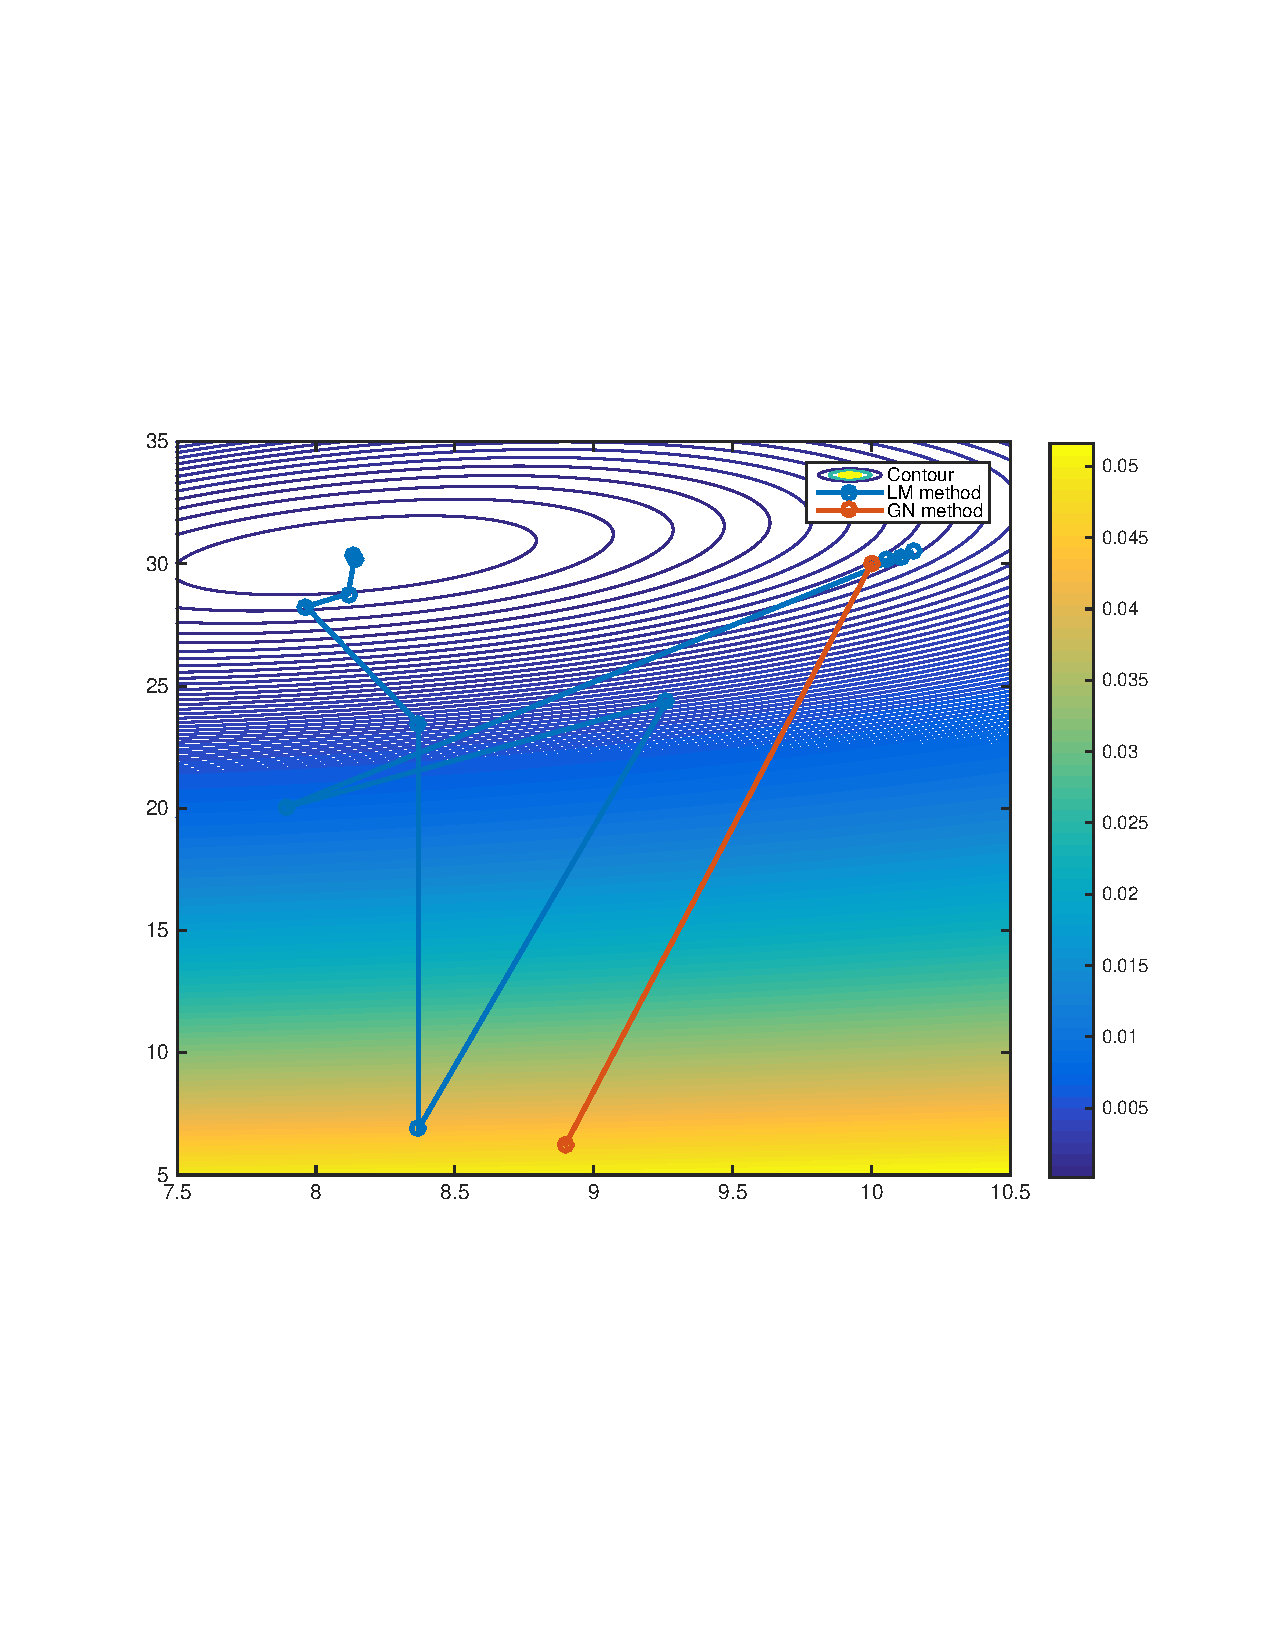
\includegraphics[width=12cm]{p1/fig1b} 
\end{figure}



\subsection*{Problem 2 (graded by Stephen) 20 points}


\subsubsection*{(a) - 5 points}

For the case of a linear regression model, we know that our G matrices
always have the form:

\[
G=\begin{pmatrix}1 & x_{1}\\
1 & x_{2}\\
1 & x_{3}\\
1 & x_{4}
\end{pmatrix}
\]


Our G matrices only know about where we took the measurements (x-values);
they don't know anything about the corresponding y-values at these
points. Thus there are infinitely many datasets that can correspond
to these G matrices. The points DO NOT need to be on a line, or even
nearly linear for that matter, for we can still find a \char`\"{}best
fit linear model\char`\"{} for any arbitrary dataset. The only requirement
is that the points be at x=1, -3, 4, 5 for $G_{1}$, x=-0.1, 0.3,
-0.4, 0.5 for $G_{2}$, and x= 101, 97, 104, 105 for $G_{3}$.

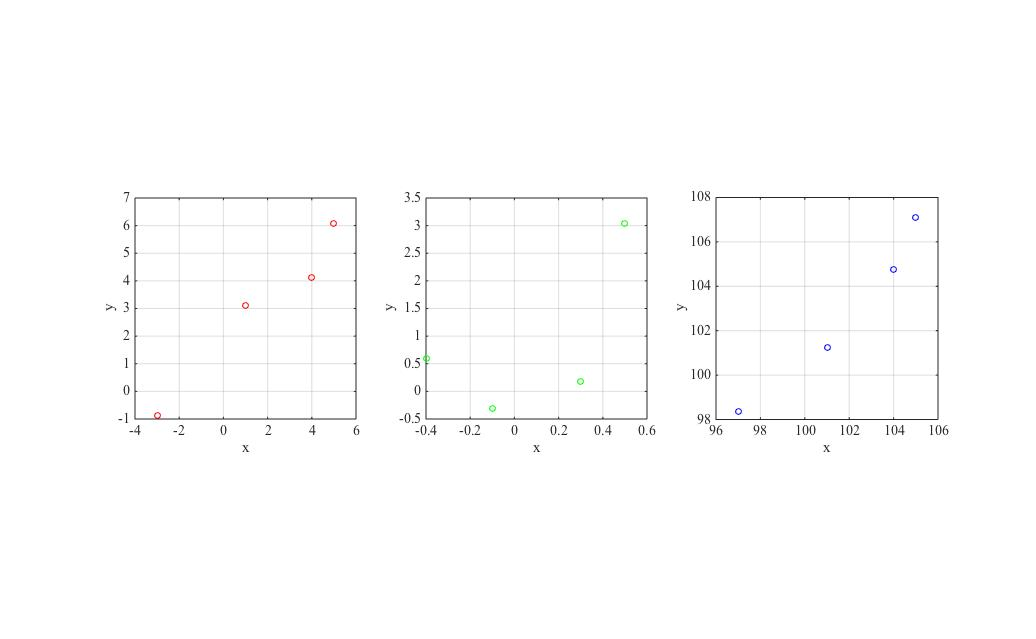
\includegraphics{p2/p21}


\subsubsection*{(b) - 5 points}

We plug in $G_{1}$, $G_{2}$, and $G_{3}$ into Matlab and simply
use the SVD function to get the singular value decompostions. See
attached matlab code after part c. The outputs are:

\[
U_{1}=\begin{pmatrix}0.1572 & 0.4897 & -0.5885 & -0.6239\\
-0.3916 & 0.8240 & 0.2055 & 0.3543\\
0.5688 & 0.2390 & 0.7102 & -0.3390\\
0.7060 & 0.1554 & -0.3272 & 0.6086
\end{pmatrix}
\]


\[
S_{1}=\begin{pmatrix}7.2125 & 0\\
0 & 1.7262\\
0 & 0\\
0 & 0
\end{pmatrix}
\]


\[
V_{1}=\begin{pmatrix}0.1442 & 0.9895\\
0.9895 & -0.1442
\end{pmatrix}
\]


\[
U_{2}=\begin{pmatrix}-0.4924 & 0.2653 & -0.8186 & -0.1304\\
-0.5093 & -0.3073 & 0.3239 & -0.7357\\
-0.4797 & 0.6948 & 0.4738 & 0.2504\\
-0.5178 & -0.5936 & 0.0210 & 0.6157
\end{pmatrix}
\]


\[
S_{2}=\begin{pmatrix}2.0064 & 0\\
0 & 0.6960\\
0 & 0\\
0 & 0
\end{pmatrix}
\]


\[
V_{2}=\begin{pmatrix}-0.9964 & 0.0850\\
-0.0850 & -0.9964
\end{pmatrix}
\]


\[
U_{3}=\begin{pmatrix}0.4961 & 0.1357 & -0.5885 & -0.6239\\
0.4764 & 0.7780 & 0.2055 & 0.3543\\
0.5108 & -0.3460 & 0.7102 & -0.3390\\
0.5157 & -0.5066 & -0.3272 & 0.6086
\end{pmatrix}
\]


\[
S_{3}=\begin{pmatrix}203.6050 & 0\\
0 & 0.0611\\
0 & 0\\
0 & 0
\end{pmatrix}
\]


\[
V_{3}=\begin{pmatrix}0.0098 & 1.0000\\
1.0000 & -0.0098
\end{pmatrix}
\]



\subsubsection*{(c) - 5 points}

We can calculate $G^{T}G$ for each of the matrices by hand. The results
are:

\[
G_{1}^{T}G_{1}=\begin{pmatrix}4 & 7\\
7 & 51
\end{pmatrix}
\]


\[
G_{2}^{T}G_{2}=\begin{pmatrix}4.00 & 0.30\\
0.30 & 0.51
\end{pmatrix}
\]


\[
G_{3}^{T}G_{3}=\begin{pmatrix}4 & 407\\
407 & 41451
\end{pmatrix}
\]


We can compare these to the orthogonal eigendecomposition discussed
in class. Here is the form of the orthogonal eigendecomposition:

\[
G^{T}G=V\Sigma^{T}U^{T}U\Sigma V^{T}=V\Sigma^{T}\Sigma V^{T}
\]


Note that $U^{T}U$ should multiply out to the identity, we can check
this within Matlab for $U_{1}$, $U_{2}$, and $U_{3}$. We also want
to show that the columns of the V matrix do indeed contain the eigenvectors
of $G^{T}G$ and that the corresponding eigenvalues are the squares
of the singular values.

If we use the eig() function in Matlab we can find the eigenvectors
and eigenvalues for each $G^{T}G$. We compare the first output to
the vectors that make up V in each case and see that they match. Then
we compare the eigenvalue output to the singular values by taking
the square root of the eigenvalues to get the singular values. They
also match in each case.
\begin{verbatim}
EIGVECTORS1 =

   -0.9895    0.1442
    0.1442    0.9895


EIG1 =

    2.9796         0
         0   52.0204


SV1 =

    1.7262         0
         0    7.2125


EIGVECTORS2 =

    0.0850   -0.9964
   -0.9964   -0.0850


EIG2 =

    0.4844         0
         0    4.0256


SV2 =

    0.6960         0
         0    2.0064


EIGVECTORS3 =

   -1.0000    0.0098
    0.0098    1.0000


EIG3 =

   1.0e+04 *

    0.0000         0
         0    4.1455


SV3 =

    0.0611         0
         0  203.6050
\end{verbatim}
\selectlanguage{english}%

\subsubsection*{(d) - 5 points}

We can see that the singular values vary for each of the G matrices
from part a. Both singular values for $G_{1}$ and $G_{2}$ are close
to each other. In each case they are only separated by 1 order of
magnitude. This is due to the fact that the measurement points (x-values)
were separated by the roughly the same order of magnitude as their
values. For example, for $G_{1}$ the measurement points are on the
order of ~1 and are separated by just 2 or 3 each. For $G_{2}$ the
measurement points are on the order of ~0.1 and are separated by
0.2 or 0.3 each.

However, the singular values for $G_{3}$ show a much greater disparity
(4 orders of magnitude). This is due to the fact that the measurement
points are on the order of ~100 but are only separated by 2 or 3
each (2 orders of magnitude difference). This can lead to difficulties
when trying to use $G_{3}$ to find a best fitting model because the
singular values are so far apart. It would be helpful in this situation
to have measured points further apart along the x-axis. A cluster
of measurements very near to each other relative to the overall data
space can lead to a great disparity in singular values. We can think
about this in the extreme case that we measure the same point (x-value)
over and over. Due to measurement error, this will return different
values. However, the G matrix will have all the same values in the
second column. When we calculate $G^{T}G$ we will see that it's columns
are not linearly independent. This means that $G^{T}G$ is not invertible
and will have one singular value that is 0.

In our problem, $G_{3}^{T}G_{3}'s$ columns are still linearly independent,
but they are much closer to linear dependence than either of the first
two cases. Thus, it gives a singular value that is much closer to
0 than the first two cases.

The V matrices are made up of two orthogonal vectors (the eigenvectors
in the model space in this case) that make the rotated axes of our
new reference frame. Thus, those eigenvectors associated with large
singular values are stably determined (well constrained) and those
associated with small singular values are not. If we look at the case
for $G_{3}$ we see that the first singular value is large and the
second is not. The eigenvector associated with the small value is:

\begin{equation}
\begin{pmatrix}1.0000\\
-0.0098
\end{pmatrix}
\end{equation}


(This is not really complete...)


\subsection*{Problem 3 (graded by Toby) 25 points}


\subsubsection*{(a)}

In the absence of testable information, our intuition should tell
us that the probabilities $p(A)$ and $p(B)$ are equal. Because the
total probability is $1$, we find 
\begin{equation}
p(A)=p(B)=\frac{1}{2}.
\end{equation}



\subsubsection*{(b)}

THe general formula for choosing $M$ items among $N$ items is given
by the binomial coefficient so that the fraction of choices is given
by 
\begin{equation}
F(M)=\frac{N!}{M!(N-M)!2^{N}}.
\end{equation}



\subsubsection*{(c)}

From high school math, we know that the binomial coefficients can
be arranged in Pascale's triangle. It is easy to see that the maximum
values in Pascale's triange are exacly the center values. Thus, the
$M$ that maximizes $F(M)$ is given by $M=N/2$. Thus, we have 
\begin{equation}
p=\frac{M}{N}=\frac{1}{2}.
\end{equation}



\subsubsection*{(d)}

Realizing that $M=pN$, the approximation can be derived by looking
at 
\begin{align}
\log(F(M)) & \approx N\log(N)-M\log(M)-(N-M)\log(N-M)-N\log(2)\\
 & =-N\log(2)+N\log(N)-Np\log(N)-Np\log(p)\\
 & -N(1-p)\log(1-p)-N(1-p)\log(N)\\
 & =N\left[-p\log(p)+(1-p)\log(1-p)\right]-N\log(2)\\
 & =NS(p)-N\log(2).
\end{align}
, where we assumed large $N,M,N-M$ (unsing Stirling's approximation
for the factorials). Thus, we can maximize $S$ with respect to $p$
instead of maximizing $F$ with respect to M.


\subsubsection*{(e)}

In order to find the maximum, we need to take the first derivative
of $S(p)$ and set it to zero. We have 
\begin{equation}
S'(p)=-[1+\log(p)-\frac{1}{1-p}+\frac{p}{1-p}-\log(1-p)]=-\log\left(\frac{p}{1-p}\right)=0.
\end{equation}
THis is equivalent to $1-p=p$, which yields $p=1/2$.In order for
this to be a maximum, we need that $S''<0$. The second derivate is
given by 
\begin{equation}
S''(p)=-\frac{1-p}{p}\frac{1-p+p}{1-p}=-\frac{1}{p}<0,\,\,\forall p>0.
\end{equation}
Thus, the maximum entropy solution is given by $p=1/2$.
\end{document}
